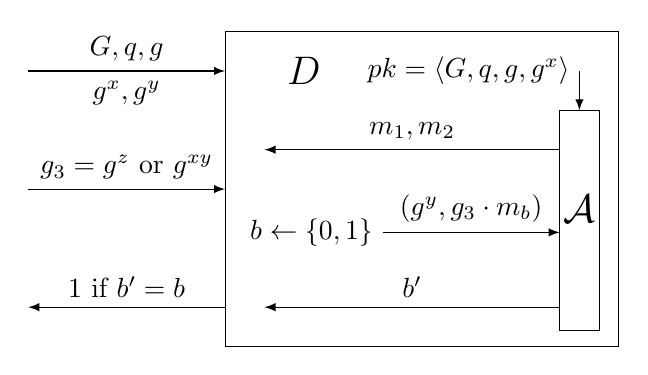
\begin{tikzpicture}
\draw (0,0) rectangle (5,4);
\draw (4.25,0.2) rectangle (4.75,3);
\draw[-latex] (-2.5,3.5) -- (0,3.5) node [midway, above] {$\mathbb{G},q,g$} node [midway, below] {$g^x, g^y$};
\draw[-latex] (-2.5,2) -- (0,2) node [midway, above] {$g_3 = g^z$ or $g^{xy}$};
%\draw[-latex] (-2.5,1.5) -- (0,1.5) node [midway, above] {$c^2_b$};
\draw[-latex] (4.5,3.5) node [left] {$pk=\langle \mathbb{G},q,g,g^x \rangle$} -| (4.5,3);
\draw[-latex] (0,0.5) -- (-2.5,0.5) node [midway, above] {1 if $b'=b$};
\draw (1,3.5) node {{\Large $D$}};
\draw (4.5,1.75) node {\Large $\mathcal{A}$};
\draw[-latex] (4.25,2.5) -- (0.5,2.5) node [midway, above] {$m_1, m_2$};
\draw[-latex] (2,1.45) node [left] {$b \gets \{0,1\}$} -- (4.25,1.45) node [midway, above] {$(g^y,g_3\cdot m_b)$};
\draw[-latex] (4.25,0.5) -- (0.5,0.5) node [midway, above] {$b'$};
%\draw[-latex] (4.5,3.5) node[above] {$pk$} -- (4.5,3);
\end{tikzpicture}